\UseRawInputEncoding

%%%%%%%%%%%%%%%%%%%%%%%%%%%%%%%%%%%%%%%%%%%%%%%%%%%%%%%%%%%%%%%%%%%%%%%%%%%%%%%%
%% Settings
%%%%%%%%%%%%%%%%%%%%%%%%%%%%%%%%%%%%%%%%%%%%%%%%%%%%%%%%%%%%%%%%%%%%%%%%%%%%%%%%
%% Columns
\documentclass[final,3p,times,twocolumn]{elsarticle}
%% Use the options 1p,twocolumn; 3p; 3p,twocolumn; 5p; or 5p,twocolumn
%% for a journal layout:
%% \documentclass[final,1p,times]{elsarticle}
%% \documentclass[final,1p,times,twocolumn]{elsarticle}
%% \documentclass[final,3p,times]{elsarticle}
%% \documentclass[final,3p,times,twocolumn]{elsarticle}
%% \documentclass[final,5p,times]{elsarticle}
%% \documentclass[final,5p,times,twocolumn]{elsarticle}
%% \documentclass[preprint,review,12pt]{elsarticle}

%% Image width
\newlength{\imagewidth}
\newlength{\imagescale}
%% preamble
\usepackage[english]{babel}
\usepackage[table]{xcolor} % For coloring tables
\usepackage{booktabs} % For professional quality tables
\usepackage{colortbl} % For coloring cells in tables
\usepackage{amsmath, amssymb} % For mathematical symbols and environments
\usepackage{amsthm} % For theorem-like environments
\usepackage{lipsum} % just for sample text
\usepackage{natbib}
\usepackage{graphicx}
\usepackage{indentfirst}
\usepackage{bashful}
\usepackage[margin=10pt,font=small,labelfont=bf,labelsep=endash]{caption}
\usepackage{graphicx}
\usepackage{calc}
\usepackage[T1]{fontenc} % [REVISED]
\usepackage[utf8]{inputenc} % [REVISED]
\usepackage{hyperref}
\usepackage{accsupp}
%% Line numbers
\linespread{1.1}
% \linenumbers
% Tables
\usepackage[pass]{geometry}
\usepackage{pdflscape}
\usepackage{csvsimple}
\usepackage{xltabular}
\usepackage{booktabs}
\usepackage{siunitx}
\usepackage{makecell}
\sisetup{round-mode=figures,round-precision=3}
\renewcommand\theadfont{\bfseries}
\renewcommand\theadalign{c}
\newcolumntype{C}[1]{>{\centering\arraybackslash}m{#1}}
\renewcommand{\arraystretch}{1.5}
\definecolor{lightgray}{gray}{0.95}

%% Diff
\usepackage{xcolor}
% Define commands for highlighting
% diff
\usepackage[most]{tcolorbox} % for boxes with transparency
% Define colors with transparency (opacity value)
\definecolor{GreenBG}{rgb}{0,1,0}
\definecolor{RedBG}{rgb}{1,0,0}
% Define tcolorbox environments for highlighting
\newtcbox{\greenhighlight}[1][]{%
  on line,
  colframe=GreenBG,
  colback=GreenBG!50!white, % 50% transparent green
  boxrule=0pt,
  arc=0pt,
  boxsep=0pt,
  left=1pt,
  right=1pt,
  top=2pt,
  bottom=2pt,
  tcbox raise base
}
\newtcbox{\redhighlight}[1][]{%
  on line,
  colframe=RedBG,
  colback=RedBG!50!white, % 50% transparent red
  boxrule=0pt,
  arc=0pt,
  boxsep=0pt,
  left=1pt,
  right=1pt,
  top=2pt,
  bottom=2pt,
  tcbox raise base
}
\newcommand{\REDSTARTS}{\color{red}}
\newcommand{\REDENDS}{\color{black}}
\newcommand{\GREENSTARTS}{\color{green}}
\newcommand{\GREENENDS}{\color{black}}
%%%%%%%%%%%%%%%%%%%%%%%%%%%%%%%%%%%%%%%%%%%%%%%%%%%%%%%%%%%%%%%%%%%%%%%%%%%%%%%%
%% Journal Name
%%%%%%%%%%%%%%%%%%%%%%%%%%%%%%%%%%%%%%%%%%%%%%%%%%%%%%%%%%%%%%%%%%%%%%%%%%%%%%%%
\journal{Heliyon}
%%%%%%%%%%%%%%%%%%%%%%%%%%%%%%%%%%%%%%%%%%%%%%%%%%%%%%%%%%%%%%%%%%%%%%%%%%%%%%%%
%% Document Starts
%%%%%%%%%%%%%%%%%%%%%%%%%%%%%%%%%%%%%%%%%%%%%%%%%%%%%%%%%%%%%%%%%%%%%%%%%%%%%%%%
\begin{document}


%%%%%%%%%%%%%%%%%%%%%%%%%%%%%%%%%%%%%%%%%%%%%%%%%%%%%%%%%%%%%%%%%%%%%%%%%%%%%%%%
%% Frontmatter
%%%%%%%%%%%%%%%%%%%%%%%%%%%%%%%%%%%%%%%%%%%%%%%%%%%%%%%%%%%%%%%%%%%%%%%%%%%%%%%%
\begin{frontmatter}
\begin{highlights}
\pdfbookmark[1]{Highlights}{highlights}

\item Neural trajectories in the hippocampus exhibited greater variability during a working memory (WM) task compared to those in the entorhinal cortex and amygdala regions.

\item The distance of neural trajectories between encoding and retrieval states in the hippocampus was memory-load dependent during a WM task.


\item Hippocampal neural trajectories fluctuated between the encoding and retrieval states in a task-dependent manner during both baseline and sharp-wave ripple (SWR) periods.

\item Hippocampal neural trajectories shifted from encoding to retrieval states during SWR period.

\end{highlights}\title{
Hippocampal neural fluctuations between memory encoding and retrieval states during a working memory task in humans: Encoding-to-retrieval shift during sharp-wave ripples
}\author[1]{Yusuke Watanabe\corref{cor1}}
\author[2,3,4]{Yuji Ikegaya}
\author[1,5]{Takufumi Yanagisawa}

\address[1]{Institute for Advanced Cocreation studies, Osaka University, 2-2 Yamadaoka, Suita, 565-0871, Osaka, Japan}
\address[2]{Graduate School of Pharmaceutical Sciences, The University of Tokyo, 7-3-1 Hongo, Tokyo, 113-0033, Japan}
\address[3]{Institute for AI and Beyond, The University of Tokyo, 7-3-1 Hongo, Tokyo, 113-0033, Japan}
\address[4]{Center for Information and Neural Networks, National Institute of Information and Communications Technology, 1-4 Yamadaoka, Suita City, 565-0871, Osaka, Japan}
\address[5]{Department of Neurosurgery, Osaka University Graduate School of Medicine, 2-2 Yamadaoka, Osaka, 565-0871, Japan}

\cortext[cor1]{Corresponding author. Tel: +81-6-6879-3652}%%Graphical abstract
%\pdfbookmark[1]{Graphical Abstract}{graphicalabstract}        
%\begin{graphicalabstract}
%\includegraphics{grabs}
%\end{graphicalabstract}
\begin{abstract}
\pdfbookmark[1]{Abstract}{abstract}
Working memory (WM) is crucial to various cognitive functions, yet its neural mechanisms remain largely elusive. Emerging interest focuses on the roles of the hippocampus and sharp wave-ripple complexes (SWRs) – transient, synchronous neural events in the hippocampus – in memory consolidation and retrieval, however, their relationship to WM tasks remains ambiguous. Recent studies propose that multiunit activity patterns in the hippocampus may operate concurrently with SWRs, exhibiting distinct dynamics during WM tasks. We performed an analysis of an electroencephalogram dataset from the medial temporal lobe (MTL) in nine patients with epilepsy during an eight-second Sternberg task. Low-dimensional neural representations, or 'trajectories', within the MTL were extracted using Gaussian-process factor analysis as the WM task was performed. The results show that significant differences in neural trajectories exist in the hippocampus compared to the entorhinal cortex and amygdala. Additionally, the divergence in trajectories between the encoding and retrieval phases appears to be memory load-dependent. Interestingly, hippocampal trajectories fluctuate during the retrieval phase, indicating task-dependent shifts between encoding and retrieval states occurring during both baseline and SWR events. These shifts from encoding to retrieval states are synchronized with the presence of SWRs, highlighting the critical function of the hippocampus in WM tasks. This finding suggests a novel hypothesis: the hippocampus modulates its functional state from encoding to retrieval in the event of SWRs.
\end{abstract}% \pdfbookmark[1]{Keywords}{keywords}                
\begin{keyword}
working memory \sep WM \sep memory load \sep hippocampus \sep sharp-wave ripples \sep SWR \sep humans
\end{keyword}
\end{frontmatter}

%%%%%%%%%%%%%%%%%%%%%%%%%%%%%%%%%%%%%%%%%%%%%%%%%%%%%%%%%%%%%%%%%%%%%%%%%%%%%%%%
%% IMRaD
%%%%%%%%%%%%%%%%%%%%%%%%%%%%%%%%%%%%%%%%%%%%%%%%%%%%%%%%%%%%%%%%%%%%%%%%%%%%%%%%
\section{Introduction}
Working memory (WM) plays a critical role in our daily activities, but the neural mechanisms underlying it are not completely understood. Particularly, the hippocampus, a key brain region involved in memory, warrants ongoing investigation \cite{scoville_loss_1957,squire_legacy_2009,boran_persistent_2019,kaminski_persistently_2017,kornblith_persistent_2017,faraut_dataset_2018,borders_hippocampus_2022,li_functional_2023,dimakopoulos_information_2022}. Enhancing our understanding of the hippocampus's role in working memory can lead to deeper insights into cognitive processes, thereby promoting the development of cognitive training strategies and interventions. 

\indent
Sharp wave ripples (SWR), transient and synchronous oscillations generated by the hippocampus, are associated with key cognitive functions, including memory replay \cite{wilson_reactivation_1994,nadasdy_replay_1999,lee_memory_2002,davidson_hippocampal_2009}, memory consolidation \cite{girardeau_selective_2009,ego-stengel_disruption_2010,fernandez-ruiz_long-duration_2019,kim_corticalhippocampal_2022}, memory recall \cite{wu_hippocampal_2017,norman_hippocampal_2019,norman_hippocampal_2021}, and neural plasticity \cite{behrens_induction_2005,norimoto_hippocampal_2018}. Consequently, SWRs could be critical to hippocampal processing and influence working memory performance. However, studies examining the influence of SWRs on working memory are scarce \cite{jadhav_awake_2012} and primarily center on rodent models utilizing navigation tasks. Such research has not clearly differentiated between the specific timing of memory recall and acquisition.

\indent
Moreover, it has been found that hippocampal neurons present low-dimensional representations during WM tasks. The firing patterns of place cells \cite{okeefe_hippocampus_1971,okeefe_place_1976,ekstrom_cellular_2003,kjelstrup_finite_2008,harvey_intracellular_2009,royer_control_2012} in the hippocampus, for instance, align with a dynamic, nonlinear three-dimensional hyperbolic geometry in rodents \cite{zhang_hippocampal_2022}. Similarly, grid cells in the entorhinal cortex (EC)—the main entry point to the hippocampus \cite{naber_reciprocal_2001,van_strien_anatomy_2009,strange_functional_2014}—display a toroidal topology during exploration \cite{gardner_toroidal_2022}. However, these studies primarily relate to spatial navigation tasks in rodents and provide limited temporal resolution for WM tasks. Additionally, it is still uncertain whether these results apply to humans or to tasks beyond navigation.

\indent
In light of these considerations, this study tests the hypothesis that hippocampal neurons demonstrate distinct low-dimensional representations, or 'neural trajectories', during WM tasks, specifically during SWR periods. To investigate this, we used a dataset of patients performing an eight-second Sternberg task (with high temporal resolution: 1 s for fixation, 2 s for encoding, 3 s for maintenance, and 2 s for retrieval) while their intracranial electroencephalography signals (iEEG) in the medial temporal lobe (MTL) were recorded \cite{boran_dataset_2020}. We implemented Gaussian-process factor analysis (GPFA) on multichannel unit activity to explore low-dimensional neural trajectories, a proven method to analyze neural population dynamics \cite{yu_gaussian-process_2009}.
\label{sec:introduction}```tex
%%%%%%%%%%%%%%%%%%%%%%%%%%%%%%%%%%%%%%%%%%%%%%%%%%%%%%%%%%%%%%%%%%%%%%%%%%%%%%%%
%% Methods
%%%%%%%%%%%%%%%%%%%%%%%%%%%%%%%%%%%%%%%%%%%%%%%%%%%%%%%%%%%%%%%%%%%%%%%%%%%%%%%%
\section{Methods}
\subsection{Dataset}
A publicly accessible dataset was utilized \cite{boran_dataset_2020}, which included nine epilepsy patients performing a modified Sternberg task comprising the subsequent four phases: fixation (1 s), encoding (2 s), maintenance (3 s), and retrieval (2 s) \cite{boran_dataset_2020}. During the encoding phase, participants were shown sets of four, six, or eight alphabetical letters, denoted herein as the set size. During the retrieval phase, participants were required to ascertain whether a probe letter had been previously shown (the correct choice for the Match IN task) or not (the correct choice for the Mismatch OUT task). Intracranial EEG (iEEG) signals were collected using depth electrodes implanted within the medial temporal lobe (MTL) regions: left and right hippocampal head (AHL and AHR), body (PHL and PHR), entorhinal cortex (ECL and ECR), and amygdala (AL and AR). These signals were recorded at a sampling rate of 32 kHz and within a frequency range of 0.5--5,000 Hz (Figure~\ref{fig:01}A and Table~\ref{tab:01}). The iEEG signals were then resampled at a rate of 2 kHz. Correlations between experimental variables such as set size and accuracy rate were uncovered (Figure~\ref{fig:s01}S1). Times of multiunit spikes were estimated using a spike sorting algorithm \cite{niediek_reliable_2016} from the Combinato package (\url{https://github.com/jniediek/combinato})(Figure~\ref{fig:01}C).

\subsection{Calculation of neural trajectories using GPFA}
To extract the neural trajectories (referred to as factors; Figure~\ref{fig:01}D) within the hippocampus, entorhinal cortex (EC), and amygdala, we employed GPFA \cite{yu_gaussian-process_2009} on multiunit activity data for each session (Figure~\ref{fig:01}D). GPFA was implemented using the elephant package (\url{https://elephant.readthedocs.io/en/latest/reference/gpfa.html}). The bin size was configured as 50 ms, with no overlaps. Each factor was z-normalized across all sessions. The Euclidean distance from the origin ($O$) was calculated based on these trajectories (Figure~\ref{fig:01}E).
\\
\indent
Within each trajectory for a region such as AHL, the \textit{geometric medians} (i.e., $\mathrm{g_{F}}$ for fixation, $\mathrm{g_{E}}$ for encoding, $\mathrm{g_{M}}$ for maintenance, and $\mathrm{g_{R}}$ for retrieval phase) were calculated by establishing the median coordinates of the trajectory during the four phases (Figure~\ref{fig:01}D). The optimal dimensionality for GPFA was defined to be three, as determined using the elbow method via log-likelihood values in a three-fold cross-validation approach (Figure~\ref{fig:02}B).

\subsection{Defining SWR candidates from hippocampal regions}
A detection method in line with the field consensus \cite{liu_consensus_2022} was used to identify potential SWR events in the hippocampus. The local field potential (LFP) signals from a region of interest (ROI), such as AHL, were re-referenced by subtracting the average signal outside the ROI (e.g., AHR, PHL, PHR, ECL, ECR, AL, AR) (see Figure~\ref{fig:01}A). These re-referenced LFP signals were used to apply a ripple-band filter (80--140 Hz) and isolate SWR-positive (SWR$^+$) candidates (see Figure~\ref{fig:01}B). SWR detection was performed using a publicly available tool (\url{https://github.com/Eden-Kramer-Lab/ripple_detection}) \cite{kay_hippocampal_2016}, with modifications such as a revised bandpass range of 80--140 Hz for human applications \cite{norman_hippocampal_2019,norman_hippocampal_2021} instead of the original 150--250 Hz range primarily used for rodents.
\\
\indent
For SWR$^+$ candidates, SWR-negative (SWR$^-$) candidates were defined as control events by shuffling the timestamps of SWR$^+$ candidates across all trials and subjects. The defined SWR$^+$/SWR$^-$ candidates were visually inspected (see Figure~\ref{fig:01}).

\subsection{Defining SWRs from putative hippocampal CA1 regions}
We confined SWR candidates within putative CA1 regions to define SWRs. First, putative CA1 regions were identified as follows. SWR$^+$/SWR$^-$ candidates within the hippocampus were embedded into a two-dimensional space based on superimposed spike counts per unit using UMAP (uniform manifold approximation and projection) \cite{mcinnes_umap_2018} in a supervised manner (Figure~\ref{fig:04}A). The silhouette score \cite{rousseeuw_silhouettes_1987}, a measure for validating clustering, was calculated from clustered samples (Table~\ref{tab:02}). Hippocampal regions showcasing an average silhouette score across sessions exceeding the 75th percentile were defined as putative CA1 regions, which resulted in five electrode locations identified from five patients (Table~\ref{tab:03}).
\\
\indent
SWR$^+$/SWR$^-$ candidates within putative CA1 regions were marked as SWRs, thereby they were no longer candidates. SWR duration and ripple band peak amplitude followed a log-normal distribution (Figure~\ref{fig:04}C \& E). As seen in Figure~\ref{fig:01}, SWR$^+$/SWR$^-$ were visually inspected. Each SWR period was divided into pre-SWR (from $-800$ to $-300$ ms from SWR center), mid-SWR (from $-250$ to $+250$ ms), and post-SWR (from $+300$ to $+800$ ms) according to the time from the center of the SWR.

\subsection{Statistical Evaluation}
The Brunner--Munzel and Kruskal-Wallis tests were conducted using the scipy package in Python \cite{virtanen_scipy_2020}. A correlation analysis was performed by determining the rank of the observed correlation coefficient in the set-size-shuffled surrogate dataset, using a custom Python script. Moreover, a bootstrap test was executed using a homemade Python script.

\label{sec:methods}
```\section{Results}
\subsection{iEEG recording and neural trajectory in MTL regions during a Sternberg task}
We employed a publicly available dataset \cite{boran_dataset_2020} for our analysis, which comprises LFP signals (Figure 1A) from MTL regions (Table~\ref{tab:01}1) recorded during a modified Sternberg task. SWR$^+$ candidates were identified in all hippocampal regions obtained from the LFP signals, filtered by the ripple band (80--140 Hz) (Figure 1B). SWR$^-$ candidates were delineated at the same timestamps as SWR$^+$ candidates but scrambled across different trials (Figure 1). The dataset also encompasses the multiunit spikes (Figure 1C), which were specified through the application of a spike sorting algorithm \cite{niediek_reliable_2016}. Using the 50-ms binned multiunit activity without overlaps, we deployed GPFA \cite{yu_gaussian-process_2009} to unravel the neural trajectory (or factors) of MTL regions by session and region (Figure 1D). Each factor was z-normalized by session and region (an example being session \#2 in AHL of subject \#1). The Euclidean distance from the origin ($O$) was then calculated (Figure 1E).

\subsection{Hippocampal neural trajectory correlation with a Sternberg task}
Figure 2A defines the median neural trajectories of 50 trials as point clouds within the three principal factor space. Using the elbow method, we established that the ideal embedding dimension for the GPFA model was three (Figure 2B). The trajectory distance from the origin ($O$) ($\mathrm{\lVert g_{F} \rVert}$, $\mathrm{\lVert g_{E} \rVert}$, $\mathrm{\lVert g_{M} \rVert}$, and $\mathrm{\lVert g_{R} \rVert}$) was larger in the hippocampus than in the EC and amygdala (Figure 2C \& D).

Similarly, the distances between geometric medians of the four phases, $\mathrm{\lVert g_{F}g_{E} \rVert}$, $\mathrm{\lVert g_{F}g_{M} \rVert}$, $\mathrm{\lVert g_{F}g_{R} \rVert}$, $\mathrm{\lVert g_{E}g_{M} \rVert}$, $\mathrm{\lVert g_{E}g_{R} \rVert}$, and $\mathrm{\lVert g_{M}g_{R} \rVert}$, were computed. It was observed that the hippocampus exhibited greater distances among the phases compared to the EC and amygdala. 

\subsection{Memory load-dependent neural trajectory distance between the encoding and retrieval states in the hippocampus}
With consideration given to the memory load of the Sternberg task, it was observed that the correct trial rate and set size (equalling the number of alphabet letter to encode) negatively correlated (Figure 3A). Similarly, a positive correlation was evident between response time and set size (Figure 3B). Also, the set size and the trajectory distance between the encoding and retrieval phases ($\mathrm{log_{10}\lVert g_{E}g_{R} \rVert}$) showed a positive relationship (Figure 3C). However, distances between other phase combinations exhibited no significant correlations (Figures 3D \& S2).

\subsection{Detection of hippocampal SWR from putative CA1 regions}
To enhance the precision of recording sites and SWR detection, we attempted to estimate electrodes in CA1 regions of the hippocampus by observing distinct multiunit spike patterns during SWR incidents. For each session and hippocampal region, SWR$^+$/SWR$^-$ candidates were embedded into a two-dimensional space using UMAP (Figure 4A). The silhouette score was determined as a measure of clustering quality (Figure 4B \& Table~\ref{tab:02}). Recording sites with an average silhouette score across sessions more significant than 0.6 were recognized as putative CA1 regions \cite{mcinnes_umap_2018, rousseeuw_silhouettes_1987}. Thus, we identified five putative CA1 regions, four of which were not previously labelled seizure onset zones (Table~\ref{tab:01}).

Next, we marked SWR$^+$/SWR$^-$ candidates within these putative CA1 regions as SWR$^+$ and SWR$^-$, respectively. Both SWR$^+$ and SWR$^-$ showed the same duration. A significant increase in SWR$^+$ incidence emerged during the initial 400 ms of the retrieval phase. Furthermore, the peak ripple band amplitude of SWR$^+$ was higher than that of SWR$^-$.

\subsection{Transient change in neural trajectory in the hippocampus during SWR}
We analyzed the \textit{distances} of the trajectory from origin ($O$) during SWR events in both encoding and retrieval phases (Figure 5A). Upon observing the increase in distance during SWR (Figure 5A), we categorized each SWR into three states: pre-, mid-, and post-SWR. 

\subsection{Visualization of hippocampal neural trajectory during SWR in two-dimensional spaces}
Based on our observations of the neural trajectory 'jump' during SWR (Figure 5), we visualized the three-dimensional trajectories of pre-, mid-, and post-SWR events during the encoding and retrieval phases (Figure 6). For this visualization, we positioned $\mathrm{g_{E}}$ at the origin (0, 0) and $\mathrm{g_{R}}$ at the coordinate ($\mathrm{\lVert g_{E}g_{R} \rVert}$, 0) in two-dimensional spaces by linearly aligning peri-SWR trajectories. 

\subsection{Fluctuating hippocampal neural trajectories between encoding and retrieval states}
Subsequently, we inspected the trajectory \textit{directions} based on $\overrightarrow{\mathrm{g_{E}g_{R}}}$. Directions of SWRs were identified by the neural trajectory at $-250$ ms and $+250$ ms from their center (i.e., $\overrightarrow{\mathrm{eSWR^+}}$). From this data, we computed the density of $\overrightarrow{\mathrm{eSWR}} \cdot \overrightarrow{\mathrm{g_{E}g_{R}}}$, $\overrightarrow{\mathrm{rSWR}} \cdot \overrightarrow{\mathrm{g_{E}g_{R}}}$, and $\overrightarrow{\mathrm{eSWR}} \cdot \overrightarrow{\mathrm{rSWR}}$ (Figure 7A--D).
    \section{Discussion}
This study hypothesized that hippocampal neurons express distinct representations, or trajectories, in low-dimensional spaces during a working memory (WM) task in humans, specifically during sharp-wave ripple (SWR) periods. Initially, we projected the multiunit spikes from medial temporal lobe regions during a Sternberg task onto three-dimensional spaces using Gaussian-process factor analysis (GPFA) (Figure~\ref{fig:01}D--E and Figure~\ref{fig:02}A) \cite{yu_gaussian-process_2009}. The trajectory distance amongst WM phases ($\mathrm{\lVert g_{F}g_{E} \rVert}$, $\mathrm{\lVert g_{F}g_{M} \rVert}$, $\mathrm{\lVert g_{F}g_{R} \rVert}$, $\mathrm{\lVert g_{E}g_{M} \rVert}$, $\mathrm{\lVert g_{E}g_{R} \rVert}$, and $\mathrm{\lVert g_{M}g_{R} \rVert}$) was larger in the hippocampus than in the entorhinal cortex (EC) and amygdala (Figure~\ref{fig:02}E), suggesting increased neural activity in the hippocampus during the WM task. Moreover, the trajectory distance between the encoding and retrieval phases in the hippocampus ($\mathrm{\lVert g_{F}g_{E} \rVert}$) displayed a positive correlation with memory load (Figure~\ref{fig:03}C--D), indicating that it reflects WM processing. The neural trajectory in the hippocampus also showed a transient increase during SWRs (Figure~\ref{fig:05}). Finally, the hippocampal neural trajectory alternated between encoding and retrieval states, transitioning from encoding to retrieval during SWR events (Figure~\ref{fig:07}). Overall, these findings emphasize the role of hippocampal neural activity in a WM task in humans \cite{naber_reciprocal_2001,van_strien_anatomy_2009,strange_functional_2014}.

We found that the distance of the neural trajectory among the four phases was longer in the hippocampus compared to the EC and amygdala, even when adjusting for the distance from origin $O$ ($\mathrm{\lVert g_{F} \rVert}$, $\mathrm{\lVert g_{E} \rVert}$, $\mathrm{\lVert g_{M} \rVert}$, and $\mathrm{\lVert g_{R} \rVert}$) in those regions (Figure~\ref{fig:02}C--E). These findings align with existing reports of hippocampal persistent firing in the maintenance phase \cite{boran_persistent_2019} \cite{kaminski_persistently_2017} \cite{kornblith_persistent_2017} \cite{faraut_dataset_2018}, reinforcing the role of the hippocampus in the WM task. Notably, by applying GPFA to multiunit activity during a one-second resolution WM task, we observed that the neural trajectory in low dimensional space exhibits a memory-load dependency between the encoding and retrieval phases, represented as $\mathrm{\lVert g_{E}g_{R} \rVert}$ (Figure~\ref{fig:03}). These results reaffirm the association between the hippocampus and WM processing \cite{oso_boran_2020}.

The reliability of our analysis, confined to presumed CA1 regions (Figure~\ref{fig:04}), is supported by several factors. This focused approach is grounded in consistent reports that SWRs are synchronous with spike bursts of interneurons and pyramidal neurons \cite{buzsaki_two-stage_1989} \cite{quyen_cell_2008} \cite{royer_control_2012} \cite{hajos_input-output_2013}, potentially within a 50 $\mu$m radius of the recording site \cite{schomburg_spiking_2012}. In this study, we noted an increase in SWR occurrences at 0--400 ms of the retrieval phase (Figure~\ref{fig:04}D), paralleling previous studies demonstrating increased SWR occurrences before spontaneous verbal recall \cite{norman_hippocampal_2019} \cite{norman_hippocampal_2021}. This finding not only corroborates earlier observations, but also broadens them by extending to a triggered retrieval stage. Additionally, the log-normal distributions of SWR duration and ripple band peak amplitude observed in this study (Figure~\ref{fig:04}C & E) are consistent with the consensus in the field \cite{liu_consensus_2022}. Therefore, our approach of restricting recording sites to probable CA1 regions likely enhanced the accuracy of SWR detection. It is essential to mention that the increase in trajectory distance from origin $O$ during SWR (Figure~\ref{fig:05}) may be slightly skewed due to the channel selection; however, this does not severely impact our primary findings.

Interestingly, trajectory directions in the retrieval phase alternated between encoding and retrieval states in both baseline and SWR periods (Figure~\ref{fig:07}C \& D). Moreover, these fluctuations transitioned from encoding to retrieval states during SWR (Figure~\ref{fig:07}E \& F). These findings concur with previous working theories suggesting SWR’s role in memory recall \cite{norman_hippocampal_2019} \cite{norman_hippocampal_2021}. Our results add to this understanding, specifying that SWRs occur when the hippocampal representation transitions from encoding to retrieval states. Hence, our findings provide novel insights into hippocampal representations: (i) neural fluctuations between encoding and retrieval states during a WM task and (ii) SWR as a mechanism enabling the transition from encoding to retrieval states \cite{buzsaki_hippocampal_2015}.

Additionally, our study uncovers WM-task-specific directions between encoding and retrieval SWRs (Figure~\ref{fig:07}E--F). Notably, encoding SWR and retrieval SWR pointed in opposing directions not during a Match IN but during a Mismatch OUT task. These findings may align with the memory engram theory \cite{liu_optogenetic_2012}. Indeed, the Match In task presented subjects with a previously seen letter, while the Mismatch OUT task introduced a new letter not shown in the encoding phase. These results suggest that SWR relates to working cognitive processes in humans.

In conclusion, our study has demonstrated that hippocampal activity oscillates between encoding and retrieval states during a WM task and shifts significantly from encoding to retrieval during SWR periods.

\label{sec:discussion}

%%%%%%%%%%%%%%%%%%%%%%%%%%%%%%%%%%%%%%%%%%%%%%%%%%%%%%%%%%%%%%%%%%%%%%%%%%%%%%%%
%% Reference Styles
%%%%%%%%%%%%%%%%%%%%%%%%%%%%%%%%%%%%%%%%%%%%%%%%%%%%%%%%%%%%%%%%%%%%%%%%%%%%%%%%
\pdfbookmark[1]{References}{references}
\bibliography{bibliography}
% Note Re-compile is required

%% Numbering Style (sorted)
\bibliographystyle{elsarticle-num}

% Author Style
% \bibliographystyle{plainnat}
% use \citet{}

%% Numbering Style (not-sorted) 
% \bibliographystyle{plainnat}
% use \cite{}




%%%%%%%%%%%%%%%%%%%%%%%%%%%%%%%%%%%%%%%%%%%%%%%%%%%%%%%%%%%%%%%%%%%%%%%%%%%%%%%%
%% Additional Information
%%%%%%%%%%%%%%%%%%%%%%%%%%%%%%%%%%%%%%%%%%%%%%%%%%%%%%%%%%%%%%%%%%%%%%%%%%%%%%%%
\pdfbookmark[1]{Additional Information}{additional_information}

\pdfbookmark[2]{Contributors}{contributors}                    
\section*{Contributors}
Y.W. and T.Y. conceptualized the study; Y.W. performed the data analysis; Y.W. and T.Y. wrote the original draft; and all authors reviewed the final manuscript.
\label{contributors}

\pdfbookmark[2]{Acknowledgments}{acknowledgments}                    
\section*{Acknowledgments}
This research was funded by a grant from the Exploratory Research for Advanced Technology (JPMJER1801).
\label{acknowledgments}

\pdfbookmark[2]{Declaration of Interests}{declaration_of_interest}                    
\section*{Declaration of Interests}
The authors declare that they have no competing interests.
\label{declaration of interests}

\pdfbookmark[2]{Data and code availability}{data_and_code_availability}                    
\section*{Data and code availability}
The data is available on G-Node (\url{https://doi.gin.g-node.org/10.12751/g-node.d76994/}). The source code is available on GitHub (\url{https://github.com/yanagisawa-lab/hippocampal-neural-fluctuation-during-a-WM-task-in-humans}).
\label{data and code availability}

\pdfbookmark[2]{Inclusion and Diversity Statement}{inclusion_and_diversity_statement}        
\section*{Inclusion and Diversity Statement}
We support inclusive, diverse, and equitable conduct of research.
\label{inclusion and diversity statement}

\pdfbookmark[2]{Declaration of Generative AI in Scientific Writing}{declaration_of_generative_ai}
\section*{Declaration of Generative AI in Scientific Writing}
The authors employed ChatGPT, provided by OpenAI, for enhancing the manuscript's English language quality. After incorporating the suggested improvements, the authors meticulously revised the content. Ultimate responsibility for the final content of this publication rests entirely with the authors.
\label{declaration of generative ai in scientific writing}

%% \pdfbookmark[2]{Appendices}{appendices}                    
%% \appendix
%% \section{}
%% \label{}


%%%%%%%%%%%%%%%%%%%%%%%%%%%%%%%%%%%%%%%%%%%%%%%%%%%%%%%%%%%%%%%%%%%%%%%%%%%%%%%%
%% Tables
%%%%%%%%%%%%%%%%%%%%%%%%%%%%%%%%%%%%%%%%%%%%%%%%%%%%%%%%%%%%%%%%%%%%%%%%%%%%%%%%
\clearpage
\section*{Tables}
\label{tables}
\pdfbookmark[1]{Tables}{tables}
\pdfbookmark[2]{ID 01}{id_01}
\begin{table*}[htbp]
\centering
\small
\begin{tabular}{*{11}{c}}
\toprule
\textbf{\thead{Subject ID}} &\textbf{\thead{# of sessions}} &\textbf{\thead{AHL}} &\textbf{\thead{AHR}} &\textbf{\thead{PHL}} &\textbf{\thead{PHR}} &\textbf{\thead{ECL}} &\textbf{\thead{ECR}} &\textbf{\thead{AL}} &\textbf{\thead{AR}} &\textbf{\thead{SOZ
}} &\\
\midrule
#1 & 4 & o & x & o & o & o & x & o & x & "AHR, LR" & 
\\
\rowcolor{lightgray}
#2 & 7 & o & o & o & o & o & o & o & o & "AHR, PHR" & 
\\
#3 & 3 & o & o & o & o & o & o & o & x & "AHL, PHL" & 
\\
\rowcolor{lightgray}
#4 & 2 & o & o & o & o & o & o & o & o & "AHL, AHR, PHL, PHR" & 
\\
#5 & 3 & o & x & x & o & x & x & o & x & DRR
\\
\rowcolor{lightgray}
#6 & 6 & o & o & o & o & o & o & o & o & "AHL, PHL, ECL, AL" & 
\\
#7 & 4 & o & o & o & o & o & o & o & o & "AHR, PHR" & 
\\
\rowcolor{lightgray}
#8 & 5 & o & o & o & o & o & o & o & o & ECR
\\
#9 & 2 & o & o & o & o & o & o & o & o & "ECR, AR" & 
\\
\bottomrule
\end{tabular}
\captionsetup{width=1\textwidth}
\caption{\textbf{
Electrode Positions in the Dataset
}
\smallskip
\\
This figure annotates the positions of the electrodes and the seizure onset zones. Regions marked with an "o" symbol are included, whereas those designated by an "x" (\textit{navy}) are omitted from the dataset. The following abbreviations are used: AHL refers to the left hippocampal head, AHR to the right hippocampal head, PHL to the left hippocampal body, PHR to the right hippocampal body, ECL to the left entorhinal cortex, ECR to the right entorhinal cortex, AL to the left amygdala, AR to the right amygdala, and SOZ to the seizure onset zone \cite{boran_dataset_2020}.
}
% width=1\textwidth
\label{tab:01}
\end{table*}
\restoregeometry
\pdfbookmark[2]{ID 02}{id_02}
\begin{table*}[htbp]
\centering
\small
\begin{tabular}{*{5}{c}}
\toprule
\textbf{\thead{Subject}} &\textbf{\thead{AHL}} &\textbf{\thead{AHR}} &\textbf{\thead{PHL}} &\textbf{\thead{PHR
}} &\\
\midrule
#1 & 0.60 ± 0.14 & n.a. & n.a. & 0.1 ± 0
\\
\rowcolor{lightgray}
#2 & 0.21 ± 0.16 & 0.17 ± 0.21 & 0.18 ± 0.22 & 0.20 ± 0.15
\\
#3 & 0.40 ± 0.42 & 0.83 ± 0.12 & n.a. & n.a.
\\
\rowcolor{lightgray}
#4 & 0.10 ± 0.00 & 0.10 ± 0.00 & 0.90 ± 0.00 & 0.10 ± 0.14
\\
#5 & n.a. & n.a. & n.a. & n.a.
\\
\rowcolor{lightgray}
#6 & 0.63 ± 0.06 & n.a. & n.a. & 0.27 ± 0.06
\\
#7 & 0.10 ± 0.00 & 0.35 ± 0.35 & 0.37 ± 0.47 & 0.10 ± 0.00
\\
\rowcolor{lightgray}
#8 & 0.13 ± 0.10 & n.a. & 0.28 ± 0.49 & n.a.
\\
#9 & n.a. & 0.85 ± 0.07 & 0.15 ± 0.07 & n.a.
\\
\bottomrule
\end{tabular}
\captionsetup{width=1\textwidth}
\caption{\textbf{
Comparative Analysis of Silhouette Scores in UMAP Clustering of $SWR^+$ and $SWR^-$ Candidates
}
\smallskip
\\
We measured the silhouette scores (mean $\pm$ SD across sessions for individual subjects) for both SWR$^+$ and SWR$^-$ candidates in UMAP clustering, derived from their underlying multispikes (Figure 4A). The mean score was registered as 0.205 (SD = 0.285), and the median fell within an inter-quartile range (IQR; Figure 4B) \cite{mcinnes_umap_2018, rousseeuw_silhouettes_1987}.
}
% width=1\textwidth

\label{tab:02}
\end{table*}
\restoregeometry
\pdfbookmark[2]{ID 03}{id_03}
\begin{table*}[htbp]
\centering
\small
\begin{tabular}{*{6}{c}}
\toprule
\textbf{\thead{Subject ID}} &\textbf{\thead{# of sessions}} &\textbf{\thead{# of trials}} &\textbf{\thead{ROI}} &\textbf{\thead{# of SWRs}} &\textbf{\thead{SWR incidence [Hz]
}} &\\
\midrule
#1 & 2 & 100 & AHL & 274 & 0.34
\\
\rowcolor{lightgray}
#3 & 2 & 97 & AHR & 325 & 0.42
\\
#4 & 2 & 99 & PHL & 202 & 0.26
\\
\rowcolor{lightgray}
#6 & 2 & 100 & AHL & 297 & 0.37
\\
#9 & 2 & 97 & AHR & 72 & 0.09
\\
\rowcolor{lightgray}
Total = 10 & Total = 493 & "Total = 1,170" & 0.30 ± 0.13 (mean ± SD)
\\
\bottomrule
\end{tabular}
\captionsetup{width=1\textwidth}
\caption{\textbf{
Number of Identified SWR Events
}
\smallskip
\\
The table presents summary statistics for the putative CA1 regions and SWRs. To reduce sampling bias, only the first two sessions (sessions #1 and #2) from each subject were used.
}
% width=1\textwidth
\label{tab:03}
\end{table*}
\restoregeometry


%%%%%%%%%%%%%%%%%%%%%%%%%%%%%%%%%%%%%%%%%%%%%%%%%%%%%%%%%%%%%%%%%%%%%%%%%%%%%%%%
%% Figures
%%%%%%%%%%%%%%%%%%%%%%%%%%%%%%%%%%%%%%%%%%%%%%%%%%%%%%%%%%%%%%%%%%%%%%%%%%%%%%%%
\clearpage
\section*{Figures}
\label{figures}
\pdfbookmark[1]{Figures}{figures}
        \clearpage
        \begin{figure*}[ht]
            \pdfbookmark[2]{ID 01}{figure_id_01}
        	\centering
            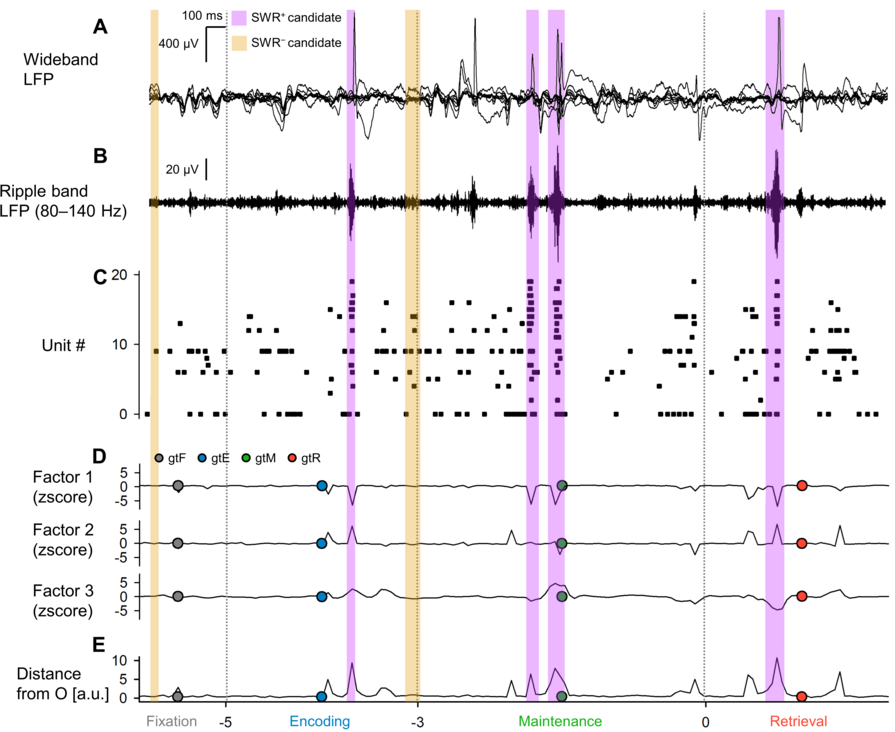
\includegraphics[width=1\textwidth]{./src/figures/.png/Figure_ID_01.png}
        	\caption{\textbf{Local Field Potential (LFP), Multiunit Activity, and Neural Trajectory of the Hippocampus during a Modified Sternberg Task} \cite{li_functional_2023, borders_hippocampal_2022, dimakopoulos_information_2022}}
\smallskip
\\
\textbf{\textit{A.}} Shown here are representative wideband LFP traces from iEEG signals, recorded from the left hippocampal head while the subject performed a modified Sternberg working memory task. The task consisted of fixation (1 s, \textit{gray}), encoding (2 s, \textit{blue}), maintenance (3 s, \textit{green}), and retrieval (2 s, \textit{red}) \cite{li_functional_2023, borders_hippocampal_2022, dimakopoulos_information_2022}. \textbf{\textit{B.}} Displayed are the associated ripple band LFP traces \cite{schomburg_spiking_2012, behrens_induction_2005, norimoto_hippocampal_2018}. \textbf{\textit{C.}} This is the raster plot of multiunit spikes, derived from the LFP traces utilizing a spike sorting algorithm \cite{niediek_reliable_2016}. \textbf{\textit{D.}} The neural trajectory, determined by GPFA, is based on the spike counts per unit with 50-ms bins \cite{yu_gaussian-process_2009}. The dotted circles symbolize the geometric median coordinates for each phase. \textbf{\textit{E.}} The trajectory distance from origin $O$ is shown. Note, the \textit{purple} and \textit{yellow} rectangles highlight the timings for SWR$^+$ candidates and SWR$^-$ candidates (controls for SWR$^+$), respectively \cite{van_vugt_hippocampal_2010, scoville_loss_1957, kay_hippocampal_2016, nader_memory_2003, wilson_reactivation_1994, nadasdy_replay_1999, lee_memory_2002}.
}
% width=1\textwidth
        	\label{fig:01}
        \end{figure*}
        \clearpage
        \begin{figure*}[ht]
            \pdfbookmark[2]{ID 02}{figure_id_02}
        	\centering
            \includegraphics[width=]{./src/figures/.png/Figure_ID_02.png}
        	\caption{\textbf{
State-dependent hippocampal neural trajectory
}
\smallskip
\\
\textbf{\textit{A.}} The figure illustrates the neural trajectory in the first three dimensions computed using the Gaussian Process Factor Analysis (GPFA). Each smaller dot represents coordinates of 50-ms neural trajectory bins, whereas larger dots outlined in \textit{black} symbolize geometric medians of consecutive phases in the Sternberg working memory task: fixation (\textit{gray}), encoding (\textit{blue}), maintenance (\textit{green}), and retrieval (\textit{red})\cite{yu_gaussian-process_2009}. \textbf{\textit{B.}} The graph reveals the log-likelihood of GPFA models in relation to the number of dimensions employed for embedding multi-unit spikes in medial temporal lobe (MTL) regions. Significantly, the dimensionality's optimal value was identified as three, determined using the elbow method\cite{virtanen_scipy_2020}. \textbf{\textit{C.}} This portion maps the distance of the neural trajectory from the origin ($O$) for the hippocampus (Hipp.), entorhinal cortex (EC), and amygdala (Amy.), and plots it against time from the probe's initiation \cite{boran_dataset_2020}. \textbf{\textit{D.}} The subsequent graph showcases the trajectory's distance from $O$ across MTL regions, with the hippocampus demonstrating the greatest distance, followed by the EC and the Amygdala\cite{fernandez-ruiz_long-duration_2019}. \textbf{\textit{E.}} The final representation indicates inter-phase trajectory distances within the MTL regions\cite{liu_consensus_2022}.
Abbreviations:
}
        	\label{fig:02}
        \end{figure*}
        \clearpage
        \begin{figure*}[ht]
            \pdfbookmark[2]{ID 03}{figure_id_03}
        	\centering
            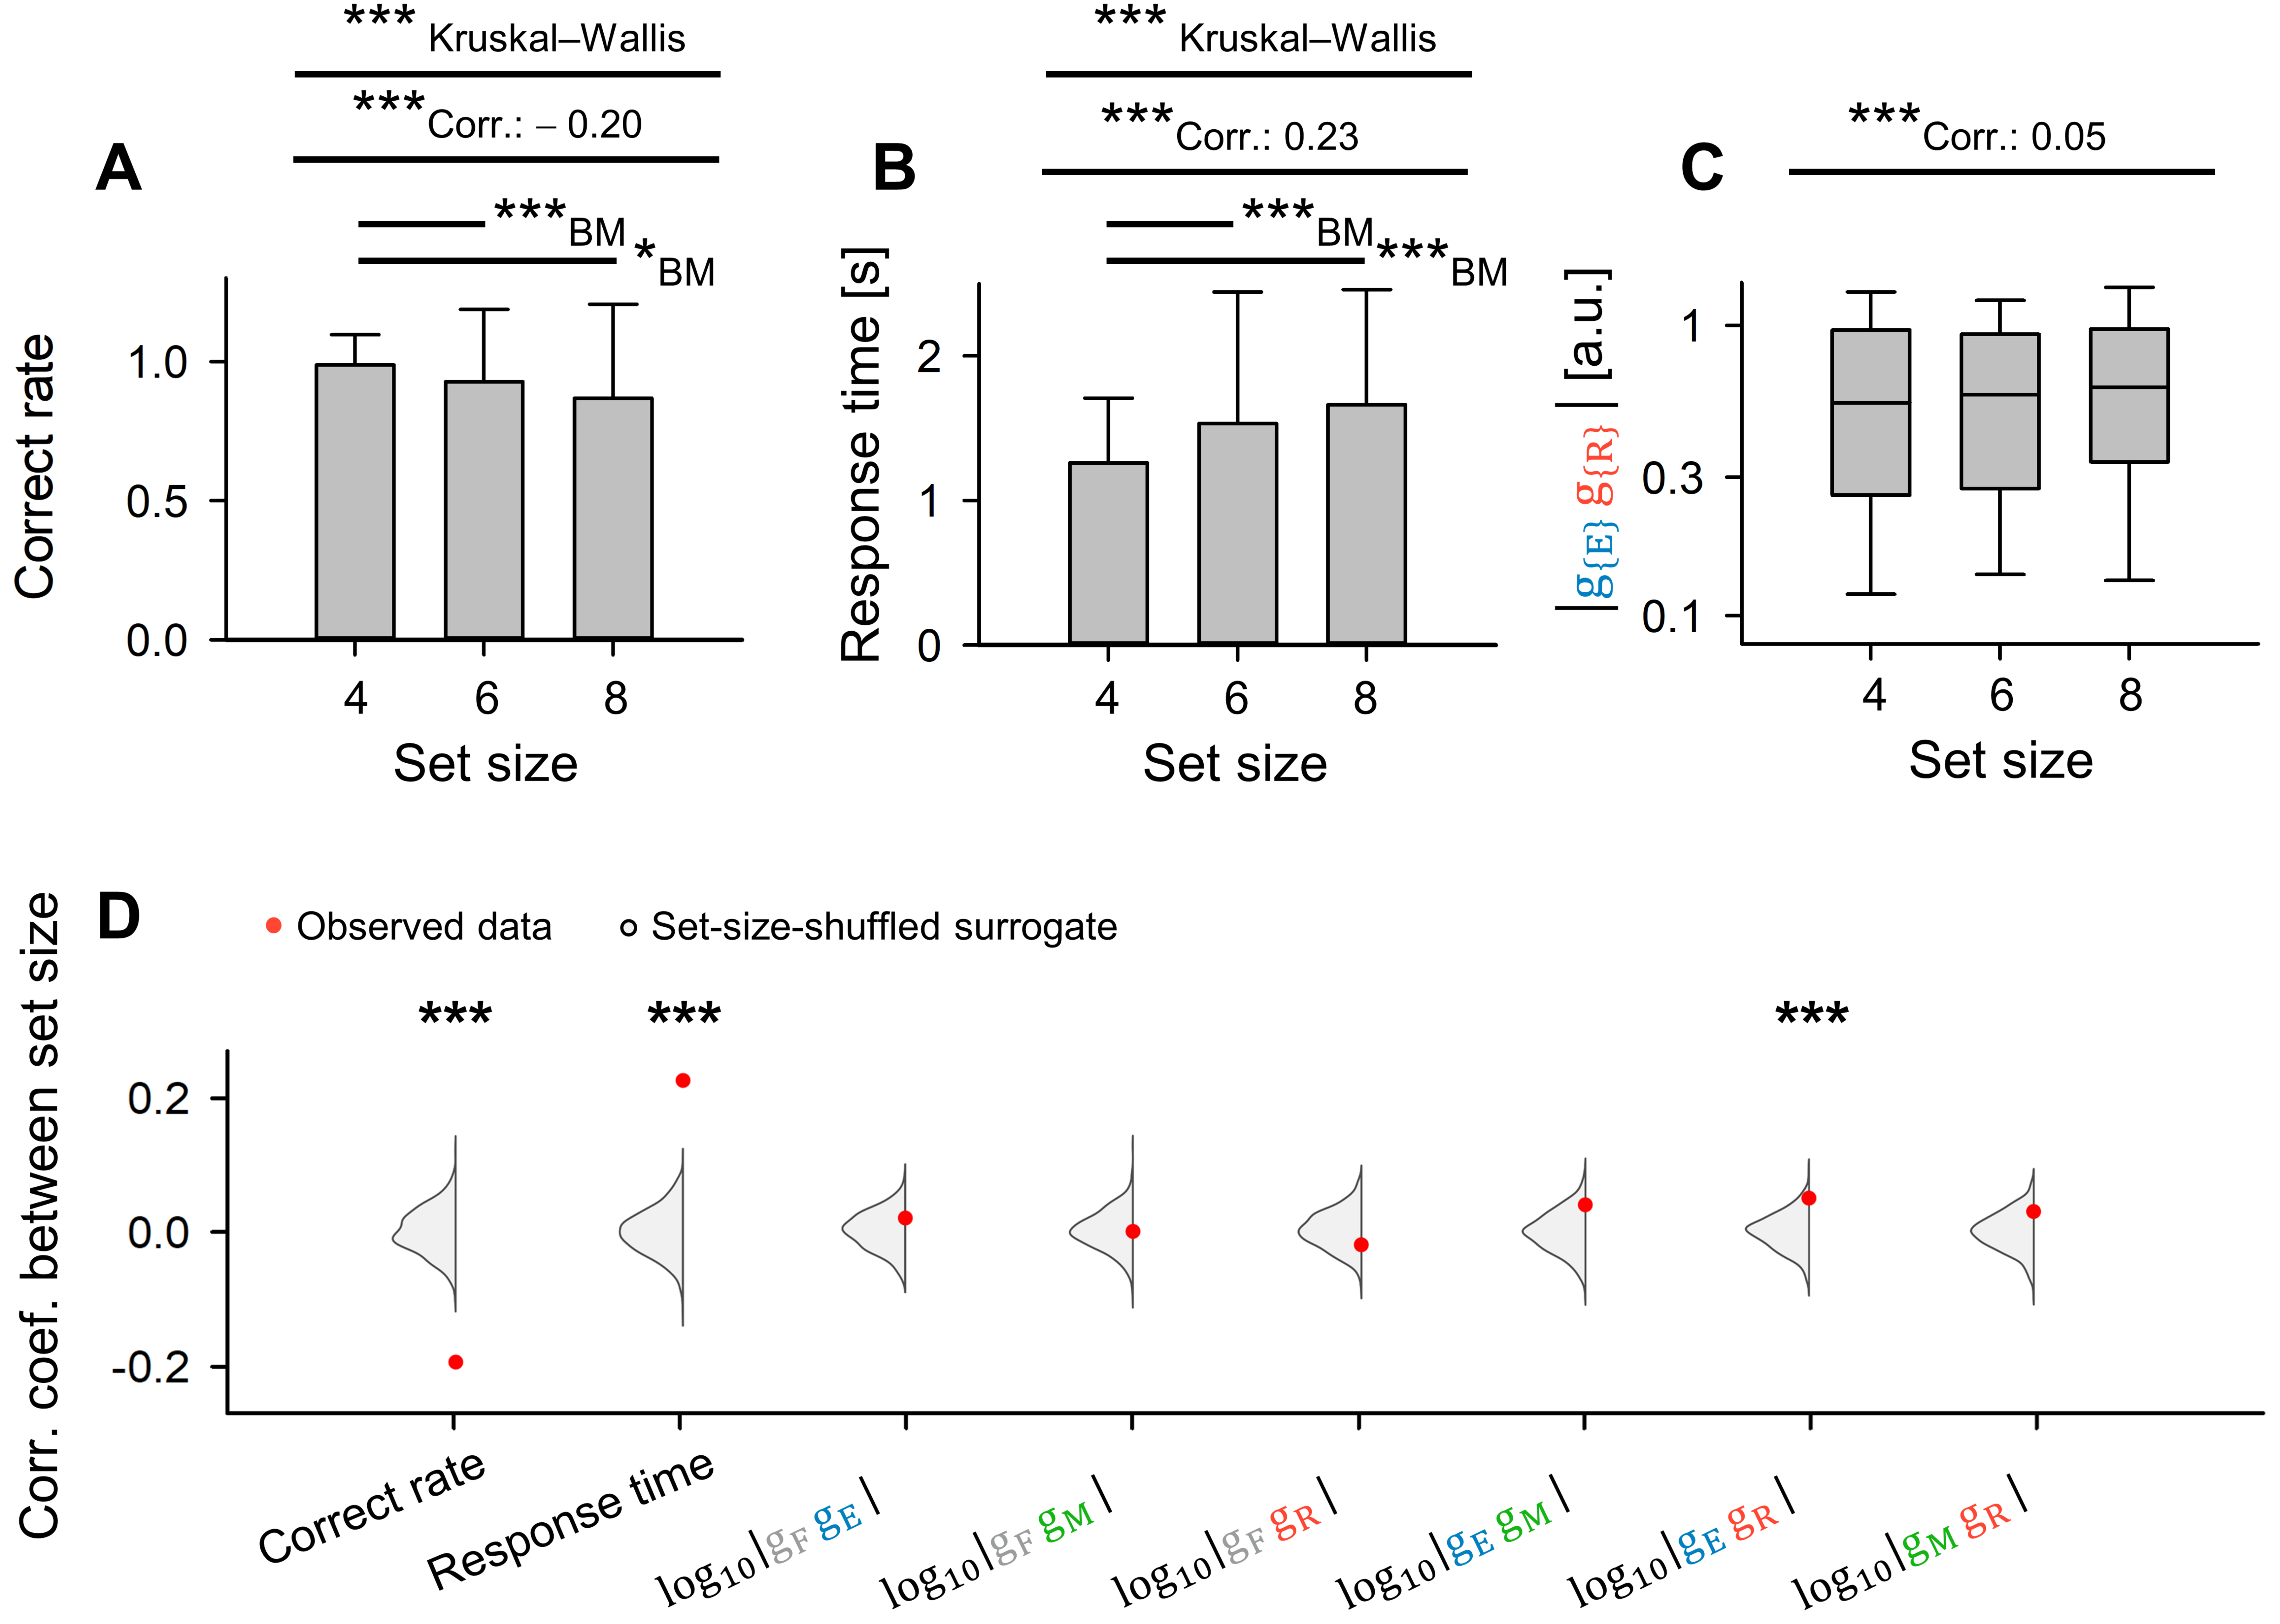
\includegraphics[width=1\textwidth]{./src/figures/.png/Figure_ID_03.png}
        	\caption{\textbf{
Dependence of Trajectory Distance on Memory Load Between Encoding and Retrieval States in the Hippocampus 
}
\smallskip
\\
\textbf{\textit{A.}} There is a significant correlation between set size (the number of letters to encode) and correct rate in the WM task (coefficient = $-0.20$, ***\textit{p} $<$ 0.001) \cite{van_vugt_hippocampal_2010, li_functional_2023, borders_hippocampus_2022}. \textbf{\textit{B.}} Set size and response time are also significantly correlated (coefficient = $0.23$, ***\textit{p} $<$ 0.001) \cite{dimakopoulos_information_2022}.  \textbf{\textit{C.}} Set size and the inter-phase distances between encoding and retrieval phases ($\Vert \mathrm{g_{E}g_{R}} \Vert$) are correlated as well, although less significantly (correlation coefficient = 0.05) \cite{li_functional_2023}. \textbf{\textit{D.}} \textit{Red} dots illustrate experimentally observed correlations between set size and the mentioned parameters: correct rate, response time, $\log_{10}{\Vert \mathrm{g_{F}g_{E}} \Vert}$, $\log_{10}{\Vert \mathrm{g_{F}g_{M}} \Vert}$, $\log_{10}{\Vert \mathrm{g_{F}g_{R}} \Vert}$, $\log_{10}{\Vert \mathrm{g_{E}g_{M}} \Vert}$, $\log_{10}{\Vert \mathrm{g_{E}g_{R}} \Vert}$, and $\log_{10}{\Vert \mathrm{g_{M}g_{R}} \Vert}$. The \textit{gray} kernel density plot indicates the corresponding set-size-shuffled surrogate measurements (\textit{n} = 1,000) (***\textit{p}s $<$ 0.001) \cite{norimoto_hippocampal_2018, hajos_input-output_2013}.
}
% width=1\textwidth
        	\label{fig:03}
        \end{figure*}
        \clearpage
        \begin{figure*}[ht]
            \pdfbookmark[2]{ID 04}{figure_id_04}
        	\centering
            \includegraphics[width=1\textwidth]{./src/figures/.png/Figure_ID_04.png}
        	\caption{\textbf{
Detection of SWRs in Assumed CA1 Regions}
\smallskip
\\
\textbf{\textit{A.}} Two-dimensional Uniform Manifold Approximation and Projection (UMAP) projection of multi-unit spikes during possible SWRs (\textit{purple}) and non-SWRs (\textit{yellow}) periods is presented\cite{mcinnes_umap_2018}. \textbf{\textit{B.}} The cumulative density plot of silhouette scores, which measure the quality of UMAP clustering, for the various hippocampal regions is plotted (see Table~\ref{tab:02}). Areas with a silhouette score above 0.60 (corresponding to the $75^{th}$ percentile) were identified as probable CA1 regions. SWR and non-SWR periods in these potential CA1 regions were defined as SWRs and non-SWRs, respectively (\textit{n}s = 1,170)\cite{rousseeuw_silhouettes_1987}. \textbf{\textit{C.}} The distribution of durations for both SWRs (\textit{purple}) and non-SWRs (\textit{yellow}) are shown, considering their respective definitions (93.0 [65.4] ms, median [IQR])\cite{girardeau_selective_2009}\cite{norman_hippocampal_2021}. \textbf{\textit{D.}} The occurrence rate of SWRs (\textit{purple}) and non-SWRs (\textit{yellow}) over time since stimulation initiation is illustrated as a mean value \textpm 95\% confidence interval. It is important to note that due to the close intervals, visualization may be difficult. Also, a significant increase in SWR occurrence was detected during the first 400 ms of the retrieval phase (0.421 [Hz], *\textit{p} < 0.05, bootstrap test)\cite{buzsaki_hippocampal_2015}\cite{ego-stengel_disruption_2010}\cite{fernandez-ruiz_long-duration_2019}. \textbf{\textit{E.}} Distributions of ripple band peak amplitudes are provided for non-SWRs (\textit{yellow}; 2.37 [0.33] SD of baseline, median [IQR]) and SWRs (\textit{purple}; 3.05 [0.85] SD of baseline, median [IQR]). Significant differences were observed (***\textit{p} < 0.001, using the Brunner--Munzel test)\cite{norman_hippocampal_2019}\cite{diba_forward_2007}\cite{liu_consensus_2022}.
}
% width=1\textwidth
        	\label{fig:04}
        \end{figure*}
        \clearpage
        \begin{figure*}[ht]
            \pdfbookmark[2]{ID 05}{figure_id_05}
        	\centering
            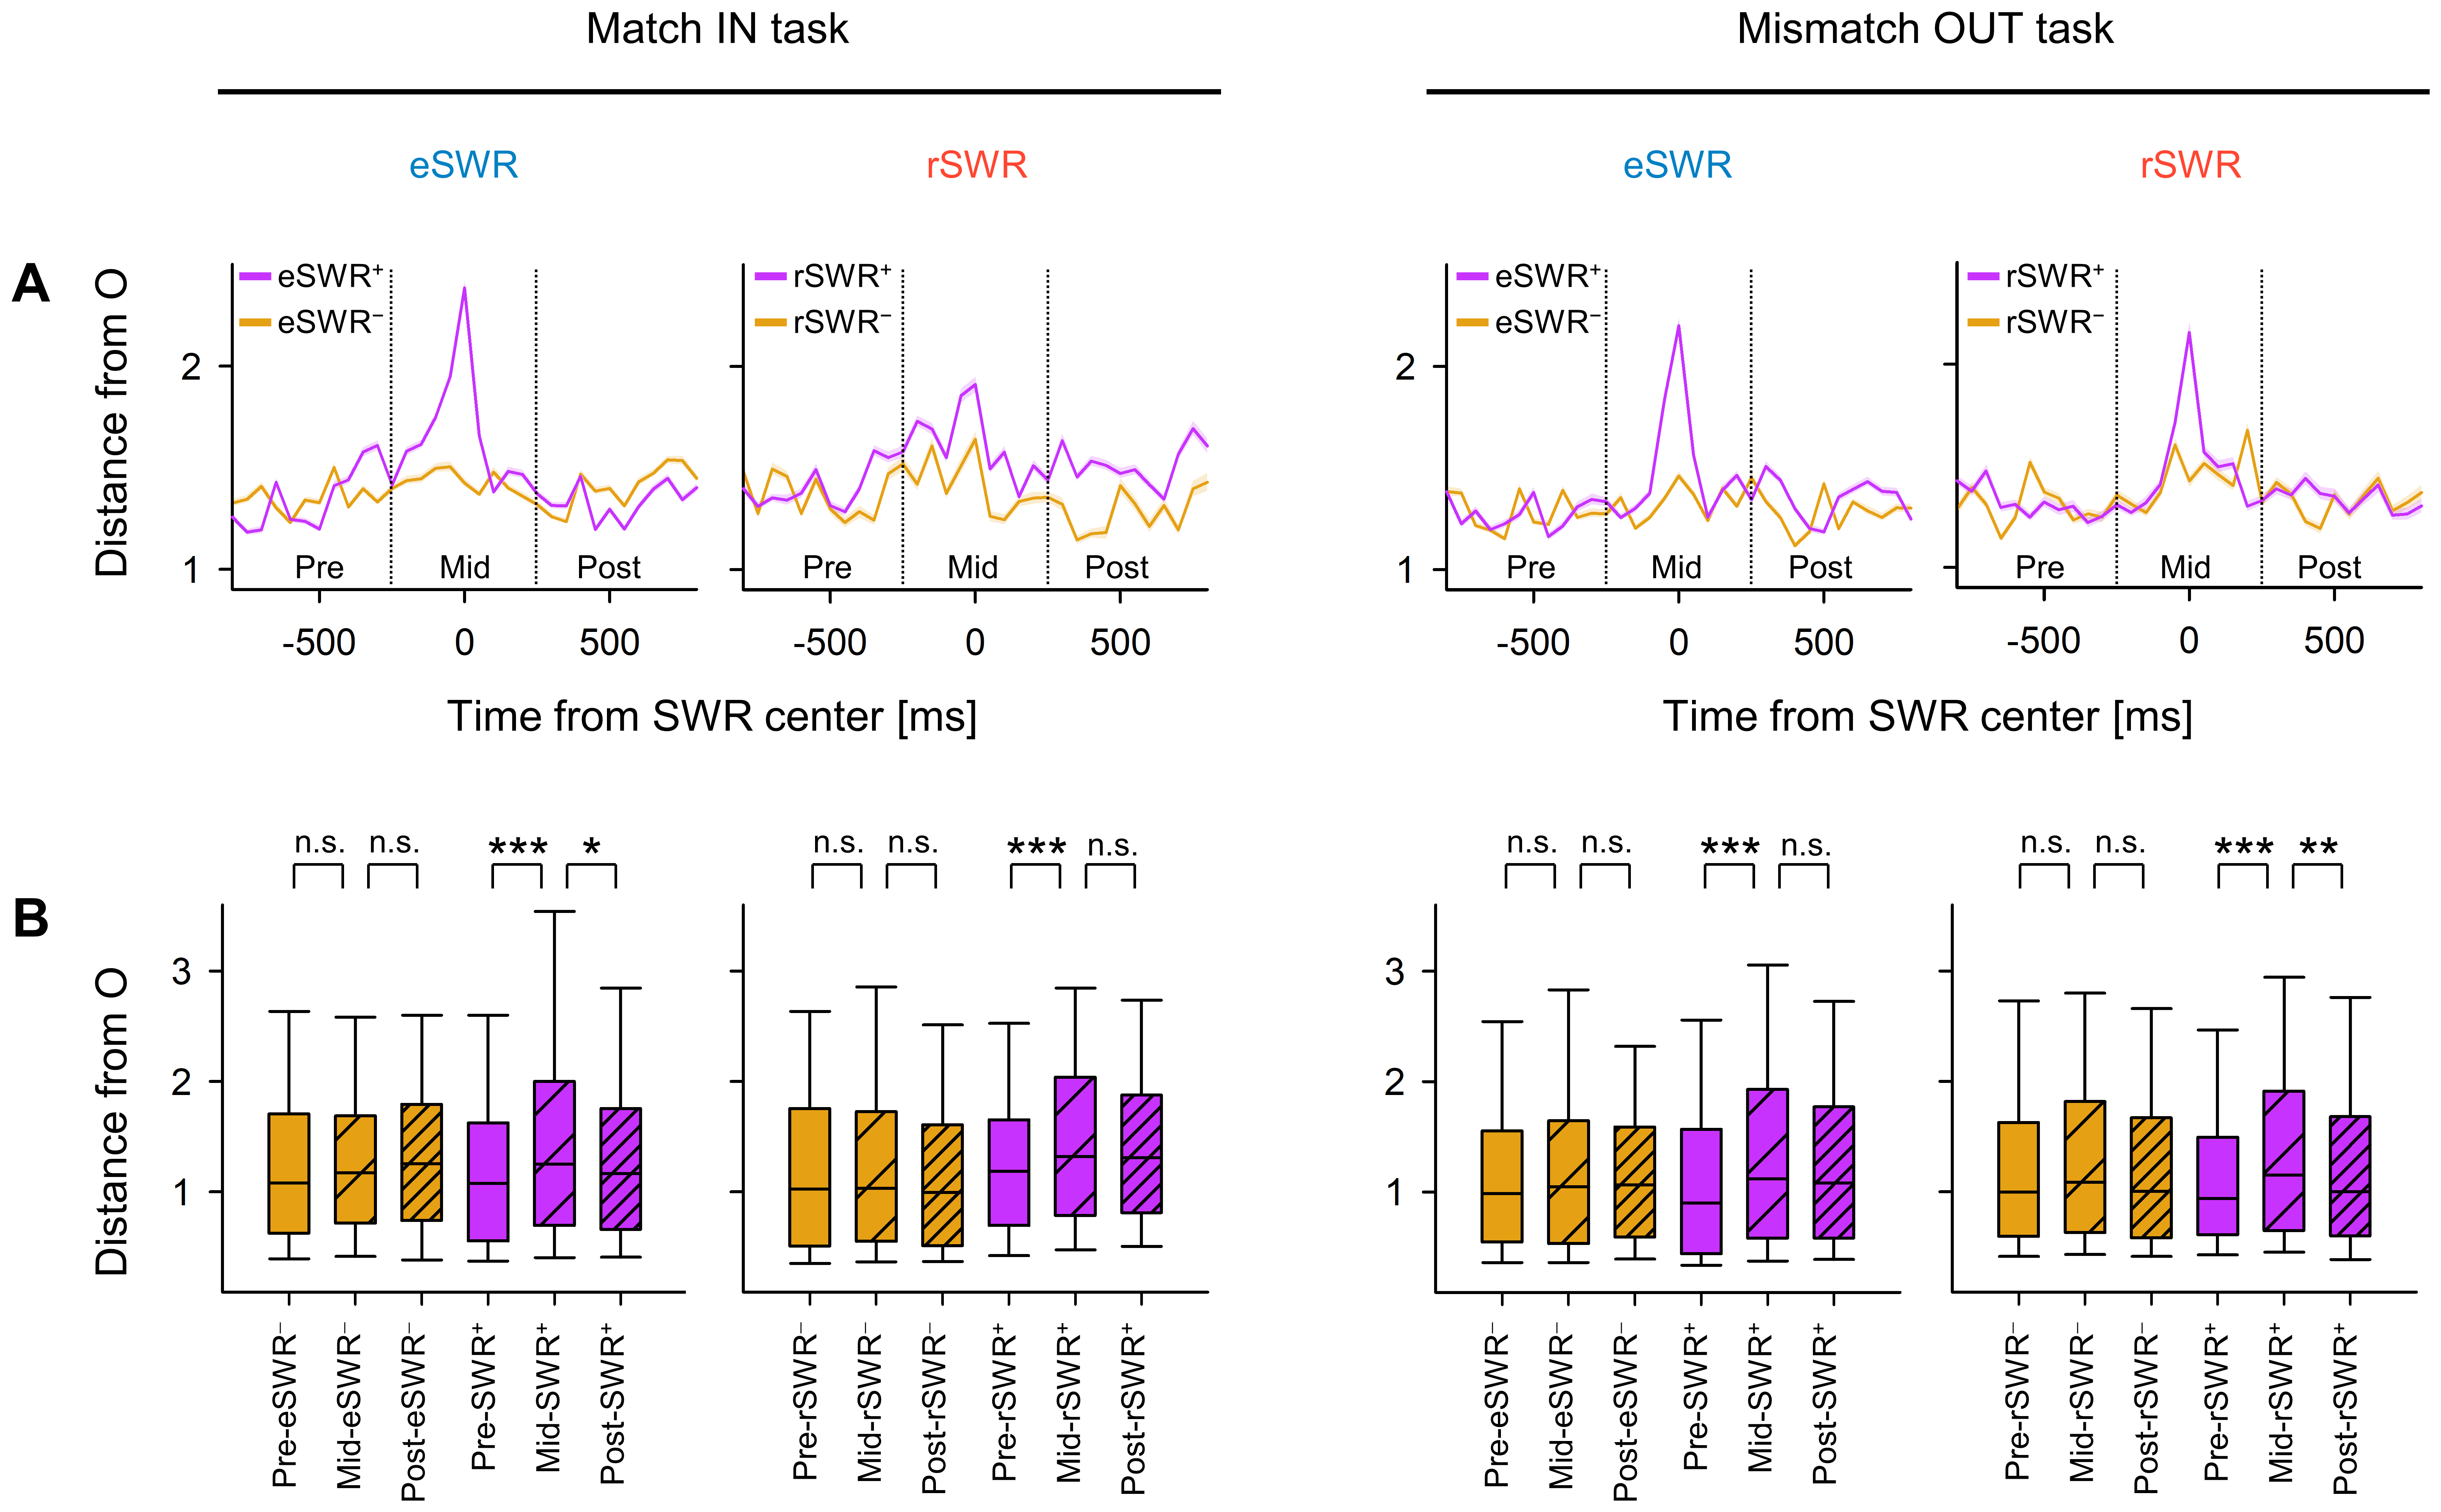
\includegraphics[width=1\textwidth]{./src/figures/.png/Figure_ID_05.png}
        	\caption{\textbf{Transient Alterations in Neural Trajectory During SWR}
\smallskip
\\
\textbf{\textit{A.}} Indicates the mean distance from the origin ($O$) of the peri-sharp-wave-ripple (SWR) trajectory, which is accompanied by a 95\% confidence interval that may not be visually detectable due to its narrow range \cite{girardeau_selective_2009,norman_hippocampal_2019,buzsaki_hippocampal_2015}. \textbf{\textit{B.}} Depicts the distance from the origin ($O$) during the pre-, mid-, and post-SWR periods (*\textit{p} $<$ 0.05, **\textit{p} $<$ 0.01, ***\textit{p} $<$ 0.001; per the Brunner--Munzel test \cite{boran_persistent_2019}). Definitions included are: SWR, sharp-wave ripple events; eSWR, SWR occurring during the encoding phase; rSWR, SWR transpiring in the retrieval phase; SWR$^+$, a SWR event; SWR$^-$, the control events paired with SWR$^+$; pre-, mid-, or post-SWR, the time intervals from $-800$ to $-250$ ms, from $-250$ to $+250$ ms, and from $+250$ to $+800$ ms, respectively, each relative to the SWR center.
}
% width=1\textwidth
        	\label{fig:05}
        \end{figure*}
        \clearpage
        \begin{figure*}[ht]
            \pdfbookmark[2]{ID 06}{figure_id_06}
        	\centering
            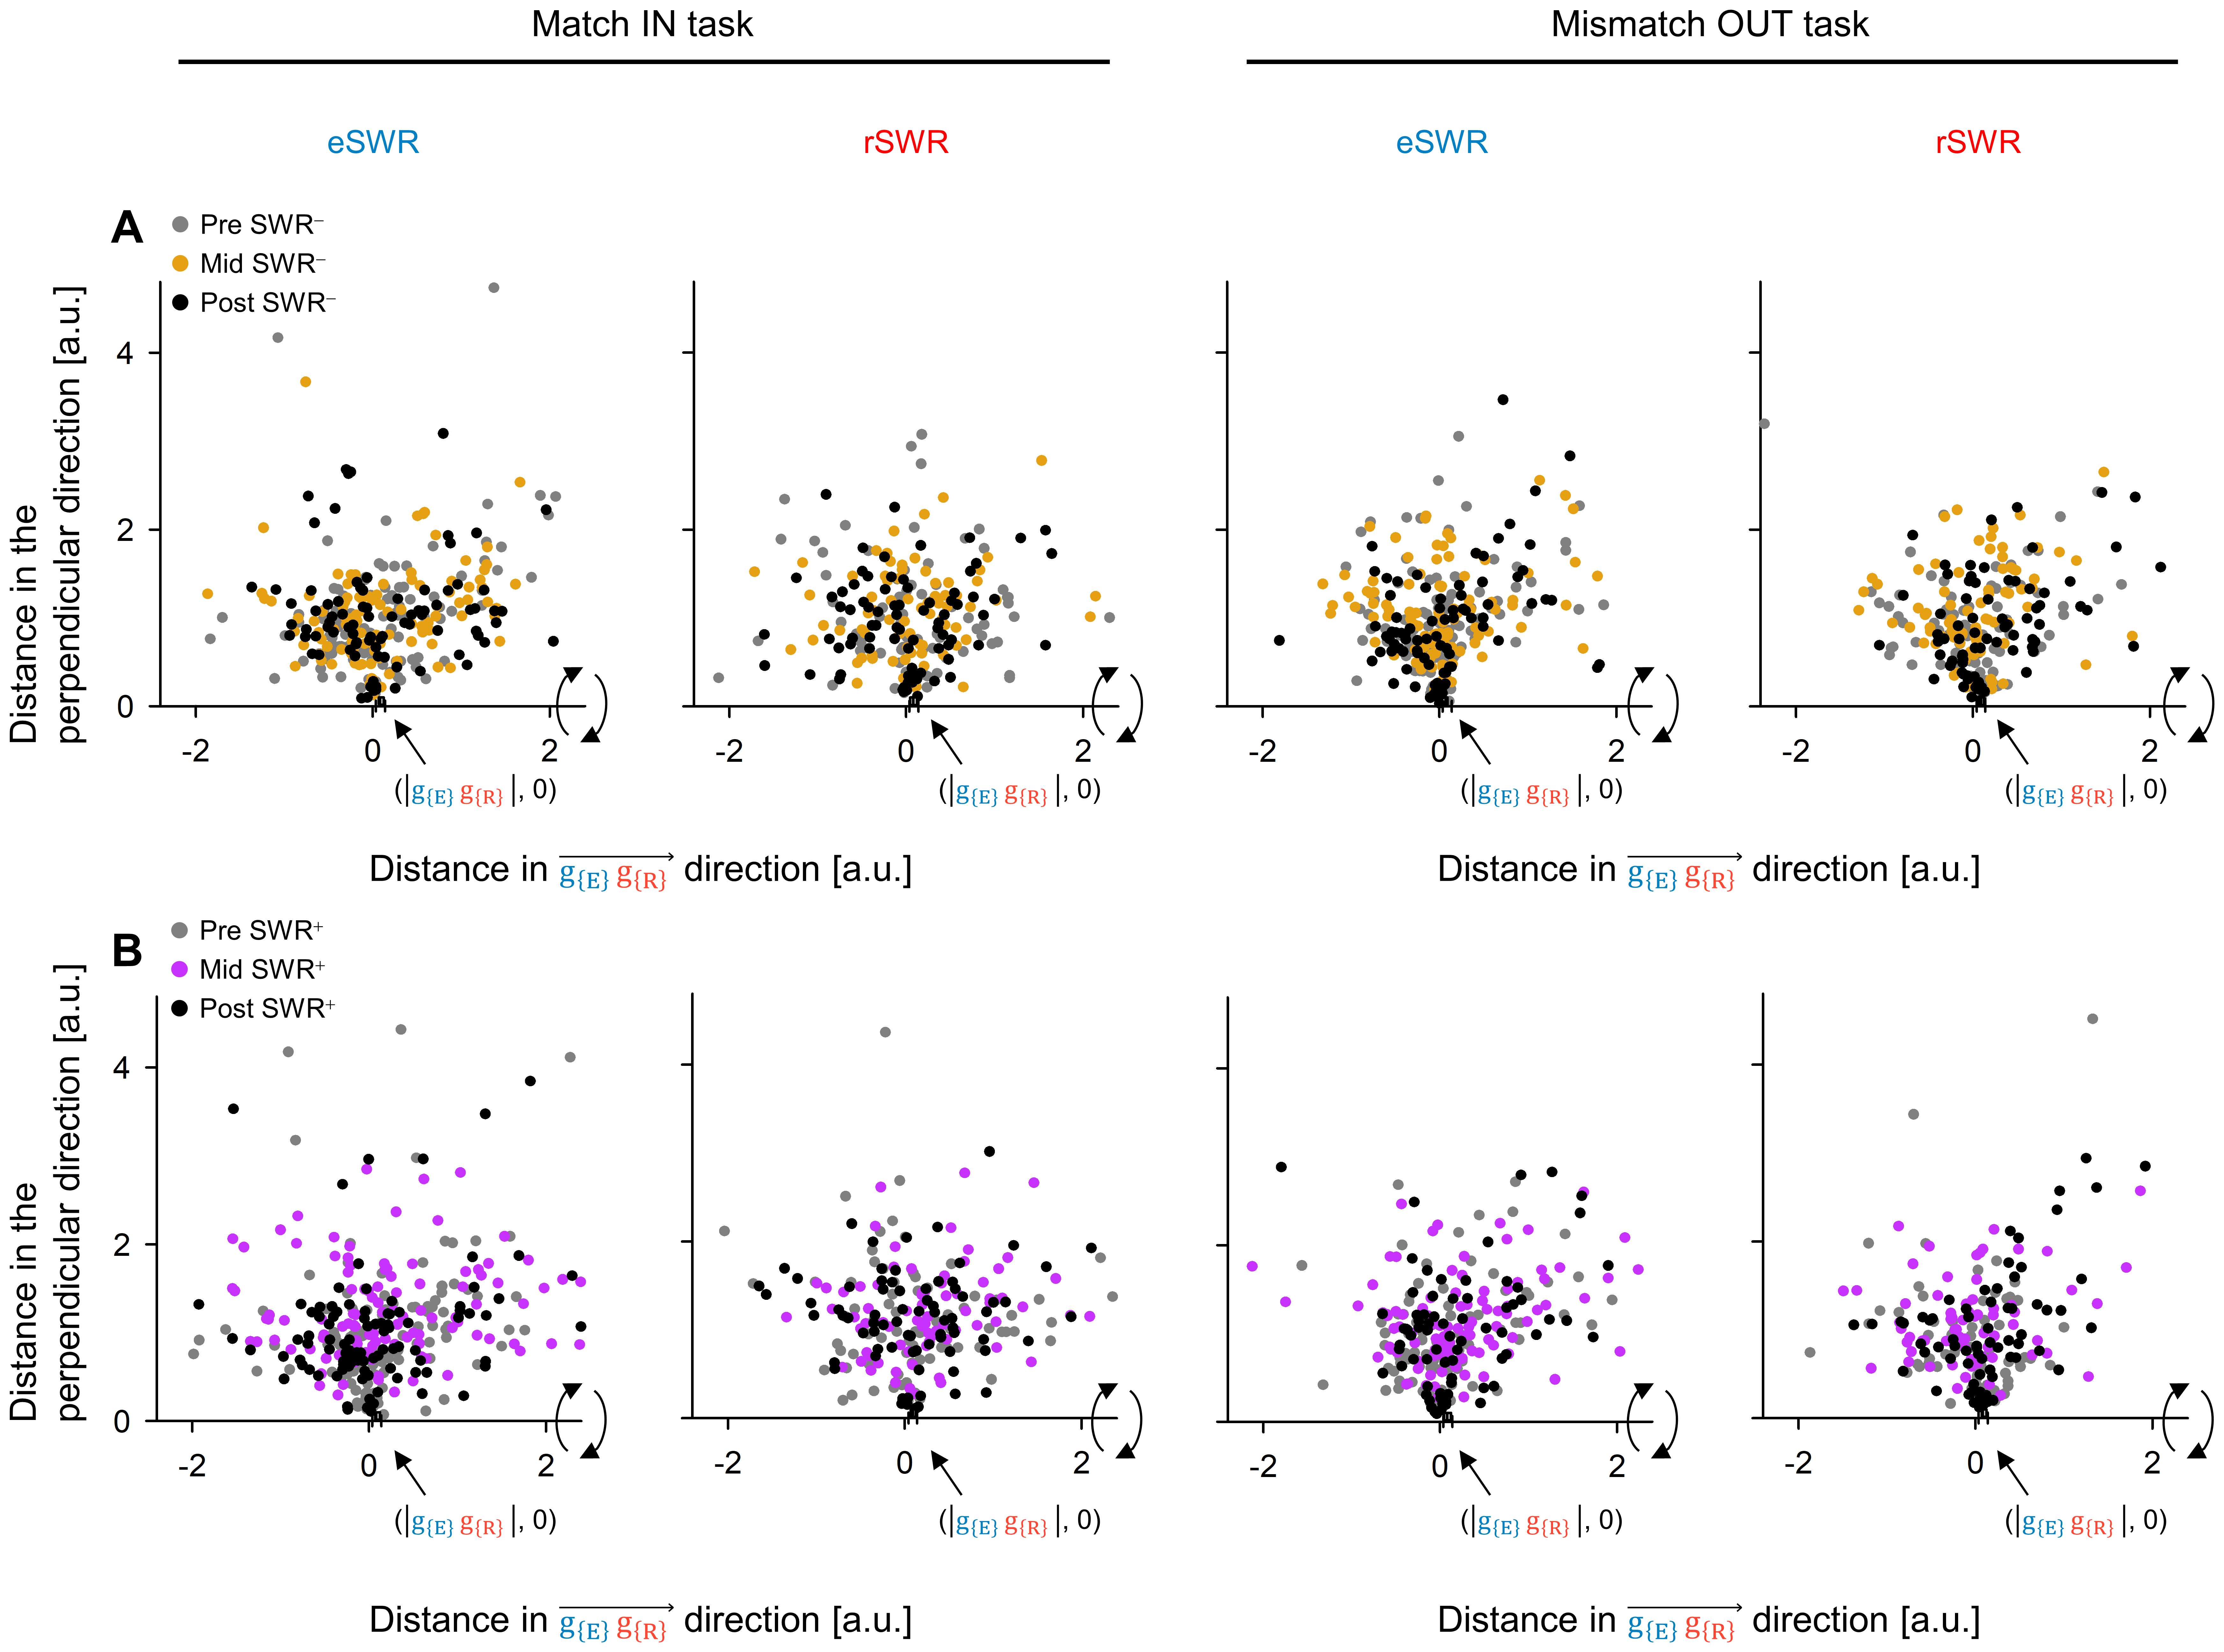
\includegraphics[width=1\textwidth]{./src/figures/.png/Figure_ID_06.png}
        	\caption{\textbf{
Visualizing Neural Trajectory During SWR in Two-Dimensional Space
}
\smallskip
\\
The presented neural trajectories pertain to hippocampal activity during Sharp-Wave Ripple (SWR) events, shown in two-dimensional space. \textbf{\textit{A.}} Trajectories representative of pre- (\textit{gray}), mid- (\textit{yellow}), and post-SWR$^-$ (\textit{black}) phases of an SWR event~\cite{buzsaki_hippocampal_2015}. \textbf{\textit{B.}} Trajectories corresponding to SWR$^+$ scenarios in contrast to SWR$^-$~\cite{fernandez-ruiz_long-duration_2019}. The magnitude of $\lVert \mathrm{g_{E}g_{R}} \rVert$ exhibits fluctuations within sessions~\cite{liu_consensus_2022}. The projecting protocol is as follows: initially, $\mathrm{g_{E}}$ was situated at the origin $O$ (0,0), and $\mathrm{g_{R}}$ at ($\lVert \mathrm{g_{E}g_{R}} \rVert$, 0) via linear transformation~\cite{kim_corticalhippocampal_2022}. Subsequently, the point cloud was rotated around the $\mathrm{g_{E}g_{R}}$ axis (the x-axis) to be compatible with a two-dimensional environment~\cite{yu_gaussian-process_2009}. Thus, both the distances from $O$ and the angles with the $\mathrm{g_{E}g_{R}}$ axis remained unaltered from their three-dimensional configuration~\cite{mcinnes_umap_2018}. Abbreviations: SWR represents Sharp-Wave Ripple events; eSWR denotes SWR during the encoding phase; rSWR signifies SWR during the retrieval phase; SWR$^+$ typifies an SWR event; SWR$^-$ signals the control events for SWR$^+$; pre-SWR, mid-SWR, or post-SWR refer to the time interval from $-800$ to $-250$ ms, from $-250$ to $+250$ ms, or from $+250$ to $+800$ ms from the center of the SWR, respectively~\cite{zhang_hippocampal_2022}.
}
% width=1\textwidth
        	\label{fig:06}
        \end{figure*}
        \clearpage
        \begin{figure*}[ht]
            \pdfbookmark[2]{ID 07}{figure_id_07}
        	\centering
            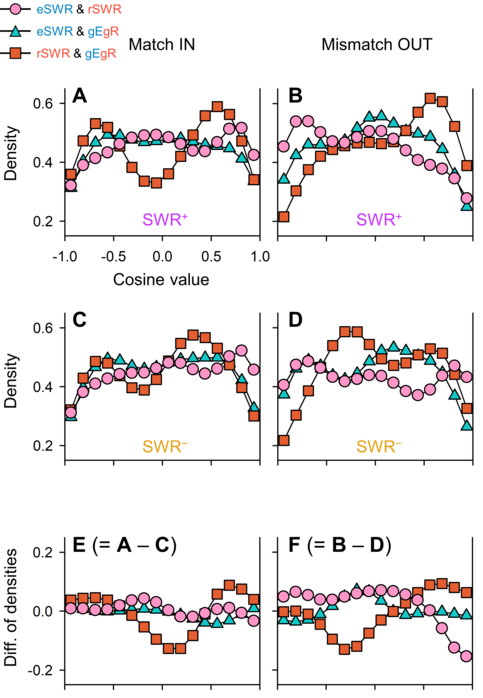
\includegraphics[width=0.5\textwidth]{./src/figures/.png/Figure_ID_07.png}
        	\caption{\textbf{
Directionality of Neural Trajectories in SWR based on Encoding and Retrieval States
}
\smallskip
\\
\textbf{\textit{A--B}} The Kernel Density Estimation (KDE) distribution of $\protect\overrightarrow{{\mathrm{eSWR^+}}} \cdot \protect\overrightarrow{{\mathrm{rSWR^+}}}$ (\textit{pink circles}), $\protect\overrightarrow{{\mathrm{eSWR^+}}} \cdot \protect\overrightarrow{{\mathrm{g_{E}g_{R}}}}$ (\textit{blue triangles}), and $\protect\overrightarrow{{\mathrm{rSWR^+}}} \cdot \protect\overrightarrow{{\mathrm{g_{E}g_{R}}}}$ (\textit{red rectangles}) in the Match IN (\textit{A}) and Mismatch OUT tasks (\textit{B}) are presented~\cite{li_functional_2023}. \textbf{\textit{C--D}} The corresponding distributions in these tasks are represented toggling $\mathrm{SWR^-}$ in place of $\mathrm{SWR^+}$~\cite{dimakopoulos_information_2022}. \textbf{\textit{E--F}} The differences between the distributions of $\mathrm{SWR^+}$ and $\mathrm{SWR^-}$ accentuate the SWR components (\textit{E} = \textit{C} $-$ \textit{A}; \textit{F} = \textit{B} $-$ \textit{D}), with the biphasic distributions of $\protect\overrightarrow{{\mathrm{rSWR^-}}} \cdot \protect\overrightarrow{{\mathrm{g_{E}g_{R}}}}$ emphasizing the neural fluctuations between encoding and retrieval states during the Sternberg task~\cite{borders_hippocampus_2022}. On the other hand, the Mismatch OUT task showed inverse directionality between $\protect\overrightarrow{{\mathrm{eSWR^+}}}$ and $\protect\overrightarrow{{\mathrm{rSWR^+}}}$ (\textit{pink circles}) which was not observed in the Match IN task (\textbf{\textit{E--F}})~\cite{naber_reciprocal_2001,van_strien_anatomy_2009}. Lastly, observed transitions from retrieval to encoding state for the SWR components occurred in both Match IN and Mismatch OUT tasks (\textit{red rectangles} in \textit{E--F})~\cite{niediek_reliable_2016,schomburg_spiking_2012}.
}
% width=0.5\textwidth
        	\label{fig:07}
        \end{figure*}


%%%%%%%%%%%%%%%%%%%%%%%%%%%%%%%%%%%%%%%%%%%%%%%%%%%%%%%%%%%%%%%%%%%%%%%%%%%%%%%%
%% END
%%%%%%%%%%%%%%%%%%%%%%%%%%%%%%%%%%%%%%%%%%%%%%%%%%%%%%%%%%%%%%%%%%%%%%%%%%%%%%%%

\end{document}
